% Provenance (never printed): see sources/outline_sources.md (Year 1:
% the Solar System, planetology). Kepler's laws, the moment of inertia and
% the Stefan--Boltzmann law are owned by the physics series and recalled
% here; the equilibrium temperature and the Bond albedo are re-founded from
% Book 2 grade 10. Curves computed in figdata/bachelor-1/planet_table.py;
% numbers of the exercises and problem in the Book 3 scratch calculator
% ch03.py.
\chapter{Comparative Planetology}\label{ch:b1:comparative-planetology}

Venus and the Earth are nearly twins: Venus has \qty{95}{\percent} of the
Earth's radius and \qty{81}{\percent} of its mass. Yet the Earth has oceans,
a nitrogen--oxygen atmosphere and moving plates, while Venus hides under
clouds a surface at \qty{737}{K}, hotter than any kitchen oven, crushed by
a carbon-dioxide atmosphere at \qty{92}{bar}. Mars, half the Earth's size,
has a thin cold atmosphere, giant volcanoes and canyons, but no moving
plates. Further out, Jupiter and Saturn
are mostly hydrogen and helium; Uranus and Neptune mostly the ices of water,
methane and ammonia. Comparing the planets is the only way to test what we
think we know about the Earth: why its interior is layered, why its climate
is mild, why it alone has plate tectonics. This chapter weighs and measures
the planets, reads their interiors from their densities and the way their
mass is distributed, compares their temperatures and atmospheres, and ends
with the moons and small bodies that keep the record of the Solar System's
youth.
% ledger: nasa:venus, earth:Rmean, earth:mass, nasa:uranus-structure

\begin{recall}
The planets go round the Sun on ellipses, and the square of a satellite's
period is proportional to the cube of its semi-major axis (Kepler's third
law, in the physics books' Year 1 volume, where the moment of inertia of a
solid is also defined; a uniform sphere has $I = \tfrac25MR^2$). A black
body radiates $\sigma T^4$ per unit area (Year 2). The Solar System and its
rocky and \omterm{def:b1:comparative-planetology:planet-types}{giant planets} were described in Book 1 (grade 6); the albedo and
the \omterm{def:b1:comparative-planetology:equilibrium-temperature}{equilibrium temperature} of a planet were met in Book 2 (grade 10), and
the greenhouse effect in Book 1 (grade 9).
\end{recall}

\begin{omfigure}
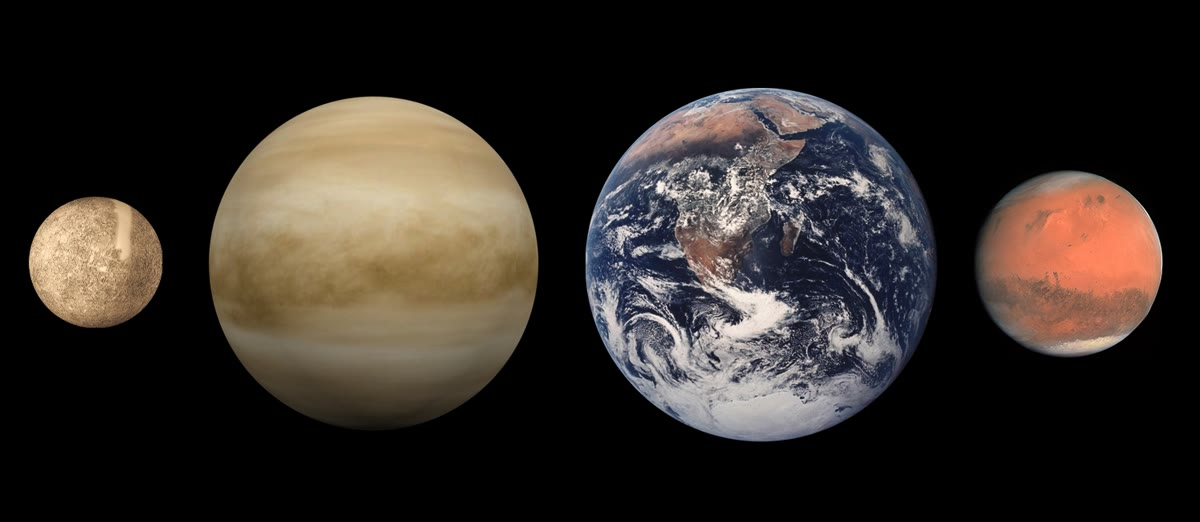
\includegraphics[width=0.85\linewidth]{images/book3/b1-terrestrial-planet-sizes.jpg}

{\small The four \omterm{def:b1:comparative-planetology:planet-types}{terrestrial planets} to scale, from left to right Mercury,
Venus, the Earth and Mars (distances not to scale; Venus as seen in visible
light, its surface hidden under clouds). NASA, public domain.}
% ledger: commons:terrestrial-sizes
\end{omfigure}

\section{Weighing and measuring the planets}

A planet's radius is measured from its angular diameter and its distance,
or, for a planet visited by spacecraft, from radar and laser altimetry. Its
mass is harder: it is felt only through the gravity the planet exerts on
something else.

\begin{method}[A planet's mass from a satellite's orbit]\label{met:b1:comparative-planetology:mass}
For a satellite of negligible mass on a near-circular orbit of radius
(semi-major axis) $a$ and sidereal period $T$ round a planet of mass $M$:
\begin{enumerate}
  \item convert $a$ to metres and $T$ to seconds;
  \item Kepler's third law gives $GM = 4\pi^2a^3/T^2$: this product is what
        the orbit measures, and to much better precision than $G$ itself;
  \item divide by $G = \qty{6.6743e-11}{m^3.kg^{-1}.s^{-2}}$ to obtain $M$.
\end{enumerate}
A planet without a moon (Mercury, Venus) is weighed in the same way from the
orbit, or the deflection, of a spacecraft that passes it.
\end{method}

\begin{example}
Io, the innermost large moon of Jupiter, orbits at $a = \qty{421.8e3}{km}$
in \num{1.769138} days, that is $T = \qty{152854}{s}$. Then
\[
  GM = \frac{4\pi^2\times(\qty{4.218e8}{m})^3}{(\qty{152854}{s})^2}
  = \qty{1.268e17}{m^3.s^{-2}}, \qquad
  M = \frac{\num{1.268e17}}{\num{6.6743e-11}} = \qty{1.900e27}{kg},
\]
which agrees with the tabulated mass of Jupiter, \qty{1.898e27}{kg}, to
\qty{0.1}{\percent}. Io's own mass, \num{4.7e-5} of Jupiter's, is negligible;
the small excess comes from Jupiter's equatorial bulge, which pulls a close
moon slightly harder than a sphere of the same mass would.
% ledger: nasa:io, nasa:jupiter, const:G
\end{example}

With the mass and the radius comes the mean density $\bar\rho =
3M/(4\pi R^3)$, the first clue to what a planet is made of. The densities of
the planets fall into two groups (see the figure below): Mercury, Venus, the
Earth and Mars lie between about \num{3900} and \qty{5500}{kg.m^{-3}},
denser than any common rock; the four outer planets lie between
\num{690} and \qty{1640}{kg.m^{-3}}, near the density of water, Saturn
even below it.
% ledger: planet:Mercury.density, planet:Mars.density, planet:Earth.density, planet:Saturn.density, planet:Neptune.density

\begin{omfigure}
\begin{tikzpicture}
\begin{axis}[omrecord, width=0.86\linewidth, height=6.2cm, xmode=log,
  xmin=800, xmax=150000, ymin=0, ymax=6300, xlabel={equatorial radius (km)},
  ylabel={mean density (\unit{kg.m^{-3}})}, tick label style={font=\scriptsize},
  label style={font=\small}]
\addplot[only marks, mark=*, mark size=2.4pt, brown!70!black] table[x=R_km, y=density,
  restrict expr to domain={\thisrow{idx}}{0:2}] {figdata/out/bachelor-1-planet_table-bodies.dat};
\addplot[only marks, mark=*, mark size=2.4pt, brown!70!black] table[x=R_km, y=density,
  restrict expr to domain={\thisrow{idx}}{4:4}] {figdata/out/bachelor-1-planet_table-bodies.dat};
\addplot[only marks, mark=*, mark size=2.4pt, orange!85!black] table[x=R_km, y=density,
  restrict expr to domain={\thisrow{idx}}{5:6}] {figdata/out/bachelor-1-planet_table-bodies.dat};
\addplot[only marks, mark=*, mark size=2.4pt, omDef] table[x=R_km, y=density,
  restrict expr to domain={\thisrow{idx}}{7:8}] {figdata/out/bachelor-1-planet_table-bodies.dat};
\addplot[only marks, mark=o, mark size=2.4pt, black!60] table[x=R_km, y=density,
  restrict expr to domain={\thisrow{idx}}{3:3}] {figdata/out/bachelor-1-planet_table-bodies.dat};
\addplot[only marks, mark=o, mark size=2.4pt, black!60] table[x=R_km, y=density,
  restrict expr to domain={\thisrow{idx}}{9:9}] {figdata/out/bachelor-1-planet_table-bodies.dat};
\addplot[black!40, densely dashed] coordinates {(800,1000) (150000,1000)};
\begin{scope}[font=\scriptsize]
\node[left] at (axis cs:2439.5,5429) {Mercury};
\node[below left] at (axis cs:6052,5243) {Venus};
\node[above] at (axis cs:6378,5514) {Earth};
\node[left] at (axis cs:3396,3934) {Mars};
\node[left] at (axis cs:1737.5,3340) {Moon};
\node[right] at (axis cs:1188,1850) {Pluto};
\node[above] at (axis cs:71492,1326) {Jupiter};
\node[left] at (axis cs:60268,687) {Saturn};
\node[right] at (axis cs:25559,1270) {Uranus};
\node[above] at (axis cs:24764,1638) {Neptune};
\node[above left, black!60] at (axis cs:150000,1000) {water};
\end{scope}
\end{axis}
\end{tikzpicture}

{\small Mean density against radius (logarithmic) for the eight planets
(filled: terrestrial, \omterm{def:b1:comparative-planetology:planet-types}{gas giants}, \omterm{def:b1:comparative-planetology:planet-types}{ice giants}), the Moon and Pluto (open
circles). Data of the NASA planetary fact sheet.}
% ledger: planet:Mercury.diameter, planet:Venus.diameter, planet:Earth.diameter, planet:Moon.diameter, planet:Mars.diameter, planet:Jupiter.diameter, planet:Saturn.diameter, planet:Uranus.diameter, planet:Neptune.diameter, planet:Pluto.diameter, planet:Mercury.density, planet:Venus.density, planet:Earth.density, planet:Moon.density, planet:Mars.density, planet:Jupiter.density, planet:Saturn.density, planet:Uranus.density, planet:Neptune.density, planet:Pluto.density
\end{omfigure}

The mean density alone cannot tell a planet made of one dense material from
a planet with a very dense centre and a lighter envelope. A second number
does: how the mass is distributed between centre and surface.

\begin{definition}[Moment-of-inertia factor]\label{def:b1:comparative-planetology:moi}
The \emph{moment-of-inertia factor}\index{moment-of-inertia factor} of a
planet is the number
\[
  C = \frac{I}{MR^2} ,
\]
where $I$ is its moment of inertia about its rotation axis, $M$ its mass and
$R$ its mean radius. A uniform sphere has $C = \tfrac25 = 0.4$; a planet
whose density increases toward the centre has $C < 0.4$, the smaller the
more the mass is concentrated.
\end{definition}

The moment of inertia is measured from the slow precession of the rotation
axis under the pull of the Sun, together with the flattening of the
planet's gravity field. The values are revealing: the Moon, $C = 0.394$, is
nearly uniform; Mars, $0.366$, and the Earth, $0.3308$, are clearly
layered; Jupiter, $0.254$, and Saturn, $0.210$, have most of their mass
packed toward their centres.
% ledger: nasa:moon, nasa:mars, earth:MoI, nasa:jupiter, nasa:saturn

\section{What the planets are made of}

\begin{definition}[Terrestrial and giant planets]\label{def:b1:comparative-planetology:planet-types}
A \emph{terrestrial planet}\index{terrestrial planet} is a planet made
mostly of silicate rock and iron, with a solid surface: Mercury, Venus, the
Earth and Mars. A \emph{giant planet}\index{giant planet} is a planet many
times more massive than the Earth, made mostly of light elements and their
compounds and without a solid surface. A \emph{gas giant}\index{gas giant}
is a giant planet made mostly of hydrogen and helium: Jupiter and Saturn.
An \emph{ice giant}\index{ice giant} is a giant planet made mostly of the
compounds astronomers call ices --- water, methane and ammonia --- under an
envelope of hydrogen and helium: Uranus and Neptune.
\end{definition}

The atmospheres the probes and telescopes measure confirm the division.
Jupiter's is \qty{89.8}{\percent} hydrogen and \qty{10.2}{\percent} helium
by volume, Saturn's \qty{96.3}{\percent} and \qty{3.25}{\percent}; for
Uranus, at least \qty{80}{\percent} of the mass is a hot dense fluid of
water, methane and ammonia above a small rocky core. A \omterm{def:b1:comparative-planetology:planet-types}{gas giant}'s mean
density stays low although its centre is strongly compressed, because hydrogen is the lightest element; an \omterm{def:b1:comparative-planetology:planet-types}{ice giant} is
denser than Saturn because its ices are heavier than hydrogen.
% ledger: nasa:jupiter, nasa:saturn, nasa:uranus-structure

The \omterm{def:b1:comparative-planetology:planet-types}{terrestrial planets} are layered as the Earth is: an iron-rich core
under a silicate mantle and a thin crust. The simplest model that uses both
measured numbers, the mean density and the \omterm{def:b1:comparative-planetology:moi}{moment-of-inertia factor}, has
two layers.

\begin{proposition}[The two-layer planet]\label{prop:b1:comparative-planetology:two-layer}
Model a planet of radius $R$ as a core of radius $xR$ and uniform density
$\rho_c$ inside a mantle of uniform density $\rho_m$. Its mean density and
its \omterm{def:b1:comparative-planetology:moi}{moment-of-inertia factor} are
\[
  \bar\rho = \rho_m + (\rho_c - \rho_m)\,x^3 , \qquad
  C = \frac25\,\frac{\rho_m + (\rho_c - \rho_m)\,x^5}{\bar\rho} .
\]
Given $\bar\rho$, $C$ and an assumed mantle density $\rho_m$, the relative
core radius follows:
\[
  x^2 = \frac{\tfrac52C\bar\rho - \rho_m}{\bar\rho - \rho_m} ,
  \qquad \rho_c = \rho_m + \frac{\bar\rho - \rho_m}{x^3} .
\]
\end{proposition}

\begin{proof}
The planet is a uniform sphere of density $\rho_m$ and radius $R$ plus a
sphere of radius $xR$ with the excess density $\rho_c - \rho_m$. Masses add:
$M = \tfrac43\pi R^3[\rho_m + (\rho_c - \rho_m)x^3]$, and dividing by the
volume gives $\bar\rho$. Moments of inertia about the same axis add too; a
uniform sphere of density $\rho$ and radius $r$ has
$I = \tfrac25\cdot\tfrac43\pi\rho r^3\cdot r^2 = \tfrac{8\pi}{15}\rho r^5$,
so $I = \tfrac{8\pi}{15}R^5[\rho_m + (\rho_c - \rho_m)x^5]$. Dividing by
$MR^2 = \tfrac43\pi\bar\rho R^5$ gives $C$. Finally the two equations read
$(\rho_c - \rho_m)x^3 = \bar\rho - \rho_m$ and $(\rho_c - \rho_m)x^5 =
\tfrac52C\bar\rho - \rho_m$; dividing the second by the first gives $x^2$,
and the first gives $\rho_c$.
\end{proof}

The model has three unknowns and two data, so one of them, the mantle
density, must be assumed from what rocks of the right composition weigh
under pressure. The answer is sensitive to that choice when $C$ is close to
$0.4$, because $\tfrac52C\bar\rho - \rho_m$ is then a small difference of
large numbers (\cref{exo:b1:comparative-planetology:10} and the problem). The
model also ignores the compression of the mantle by its own weight, which
in a planet as large as the Earth raises the density of the deep mantle well
above that of surface rocks; for the Earth, seismology does far better
(\cref{ch:b1:layered-earth}). Seismometers placed on Mars have now done the
same for that planet: where the planetary table gives a core radius of
\qty{1830}{km}, recent results indicate only \qty{1650}{km} to
\qty{1675}{km}.
% ledger: nasa:mars-core

\begin{omfigure}
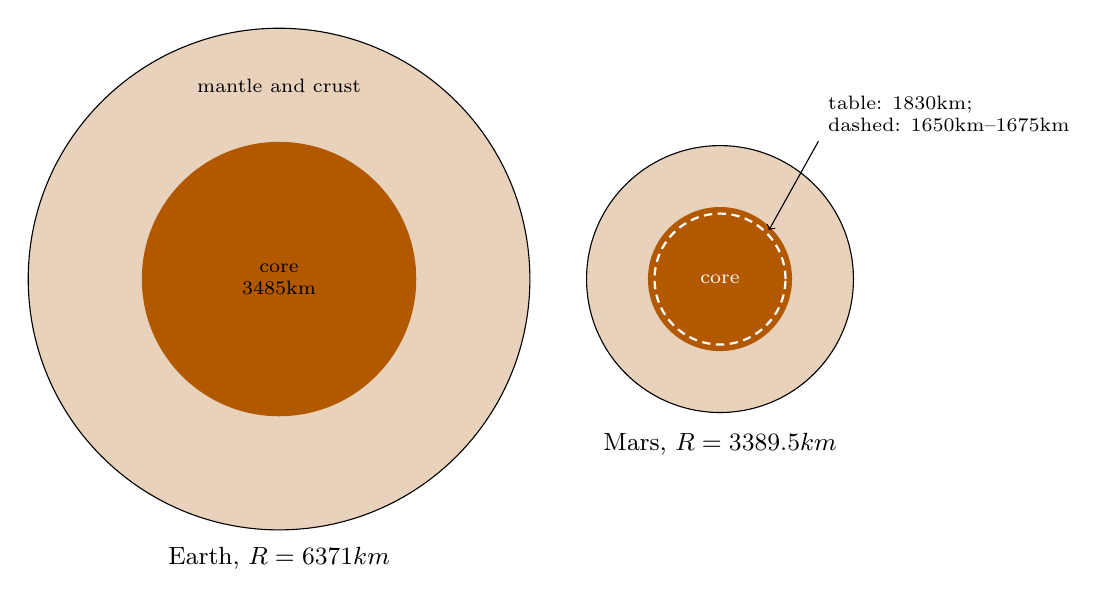
\begin{tikzpicture}[font=\scriptsize]
% scale: 0.5 cm per 1000 km
\fill[brown!35] (0,0) circle (3.1855cm);
\fill[orange!70!black] (0,0) circle (1.7425cm);
\draw (0,0) circle (3.1855cm);
\node[align=center] at (0,0) {core\\ \qty{3485}{km}};
\node[align=center] at (0,2.45) {mantle and crust};
\node at (0,-3.55) {\small Earth, $R = \qty{6371}{km}$};
\begin{scope}[xshift=5.6cm]
\fill[brown!35] (0,0) circle (1.6948cm);
\fill[orange!70!black] (0,0) circle (0.915cm);
\draw[white, densely dashed, thick] (0,0) circle (0.8313cm);
\draw (0,0) circle (1.6948cm);
\node[align=center, white] at (0,0) {core};
\node at (0,-2.1) {\small Mars, $R = \qty{3389.5}{km}$};
\draw[->] (1.25,1.75) node[above right, align=left] {table: \qty{1830}{km};\\ dashed: \qty{1650}{km}--\qty{1675}{km}} -- (0.62,0.62);
\end{scope}
\end{tikzpicture}

{\small The Earth and Mars to scale, with their cores. For Mars, the solid
edge is the core radius of the planetary table and the dashed circle the
smaller radius indicated by recent seismic results. Both cores are iron-rich;
the Earth's has a solid inner part, not drawn.}
% ledger: earth:Rmean, earth:Rcore, nasa:mars, nasa:mars-core
\end{omfigure}

\section{Atmospheres and surfaces}

A planet's temperature is set first by the sunlight it absorbs. The
irradiance $S$ at its distance $d$ from the Sun falls as $1/d^2$
(\cref{prop:b1:observing-the-sky:inverse-square}): \qty{1361}{W.m^{-2}} at
the Earth, \qty{2601}{W.m^{-2}} at Venus, \qty{586}{W.m^{-2}} at Mars,
\qty{50}{W.m^{-2}} at Jupiter. Part of it is reflected straight back.
% ledger: earth:TSI, nasa:venus, nasa:mars, nasa:jupiter

\begin{definition}[Bond albedo]\label{def:b1:comparative-planetology:albedo}
The \emph{Bond albedo}\index{Bond albedo} $A$ of a planet is the fraction
of the total power of the sunlight falling on it that it reflects and
scatters back to space, over all wavelengths and all directions.
\end{definition}

Fresh snow and bright clouds reflect much, dark rock and open sea little.
Venus, wrapped in bright clouds, has $A = 0.77$; the Earth $0.294$; Mars
$0.250$; the Moon, dark grey rock, $0.11$.
% ledger: nasa:venus, earth:albedo, nasa:mars, nasa:moon

\begin{definition}[Equilibrium temperature]\label{def:b1:comparative-planetology:equilibrium-temperature}
The \emph{equilibrium temperature}\index{equilibrium temperature} $T_\mathrm{eq}$
of a planet is the uniform temperature at which a black body of the
planet's size would radiate to space exactly the power the planet absorbs
from the Sun.
\end{definition}

\begin{proposition}[Equilibrium temperature]\label{prop:b1:comparative-planetology:teq}
A planet of \omterm{def:b1:comparative-planetology:albedo}{Bond albedo} $A$ receiving the irradiance $S$ has
\[
  T_\mathrm{eq} = \left(\frac{S(1 - A)}{4\sigma}\right)^{1/4},
  \qquad \sigma = \qty{5.6704e-8}{W.m^{-2}.K^{-4}} .
\]
\end{proposition}

\begin{proof}
The planet intercepts the sunlight falling on its cross-section, a disc of
area $\pi R^2$, and absorbs the fraction $1 - A$: it absorbs $S(1 - A)\pi
R^2$. A black body (Stefan--Boltzmann law, admitted from the physics books'
Year 2 volume) at uniform temperature $T$ radiates $\sigma T^4$ from each
square metre of its whole surface, $4\pi R^2$. Equating the two powers,
$4\pi R^2\sigma T^4 = S(1 - A)\pi R^2$, and the factor 4 is the ratio of
the sphere's area to its cross-section.
\end{proof}

With the values above, $T_\mathrm{eq}$ is \qty{255}{K} for the Earth,
\qty{227}{K} for Venus, \qty{210}{K} for Mars and \qty{270}{K} for the Moon.
Venus, though nearer the Sun, comes out colder than the Earth: its clouds
reflect three quarters of the sunlight. The figure below sets these values
beside the measured mean surface temperatures. The differences are the
greenhouse effect, which the next paragraphs and the climate chapters
(\cref{ch:b1:radiation-heat-transport}) make quantitative: about \qty{33}{K}
for the Earth, about \qty{510}{K} for Venus, only about \qty{4}{K} for Mars.
% ledger: const:sigma, earth:Tsurf, nasa:venus, nasa:mars, planet:Moon.Tmean

\begin{omfigure}
\begin{tikzpicture}
\begin{axis}[ybar, bar width=12pt, width=0.72\linewidth, height=5.8cm,
  ymin=0, ymax=820, xmin=-0.6, xmax=3.6, xtick={0,1,2,3},
  xticklabels={Moon, Mars, Earth, Venus}, ylabel={temperature (K)},
  tick label style={font=\scriptsize}, label style={font=\small},
  ymajorgrids, grid style={black!12}, axis lines*=left,
  legend style={font=\scriptsize, at={(0.03,0.97)}, anchor=north west, draw=none},
  nodes near coords, nodes near coords style={font=\tiny},
  every node near coord/.append style={/pgf/number format/fixed, /pgf/number format/precision=0}]
\addplot[fill=omDef!55, draw=omDef] table[x=idx, y=Teq] {figdata/out/bachelor-1-planet_table-temps.dat};
\addplot[fill=omThm!60, draw=omThm] table[x=idx, y=Tsurf] {figdata/out/bachelor-1-planet_table-temps.dat};
\legend{equilibrium temperature, mean surface temperature}
\end{axis}
\end{tikzpicture}

{\small \omterm{def:b1:comparative-planetology:equilibrium-temperature}{Equilibrium temperature} (computed from the irradiance and the \omterm{def:b1:comparative-planetology:albedo}{Bond
albedo}) and measured mean surface temperature of four bodies. The
atmosphere warms the Earth and above all Venus; Mars's thin atmosphere does
little; the airless Moon is colder, on average, than its \omterm{def:b1:comparative-planetology:equilibrium-temperature}{equilibrium
temperature}.}
% ledger: nasa:moon, nasa:mars, earth:TSI, earth:albedo, earth:Tsurf, nasa:venus, planet:Moon.Tmean, const:sigma
\end{omfigure}

The Moon's mean temperature, about \qty{253}{K}, falls below its
\omterm{def:b1:comparative-planetology:equilibrium-temperature}{equilibrium temperature}. This is no paradox: without an atmosphere or an
ocean to carry heat, the day side is very hot and the night side very cold,
and since emission grows as $T^4$, a body with uneven temperatures
radiates the absorbed power with a lower mean temperature than a uniform
one (\cref{exo:b1:comparative-planetology:11}).

An atmosphere does two things: it lets most of the sunlight through and it
absorbs part of the infrared the ground emits, re-emitting some of it
downward. How much it warms the surface depends on how much absorbing gas
lies above each square metre. The surface pressure measures exactly that:
$p = mg$ for a column of mass $m$ per square metre. Venus's atmosphere, at
\qty{92}{bar}, is \qty{96.5}{\percent} carbon dioxide; Mars's, at only
\qty{6.36}{mbar} on average, is \qty{95.1}{\percent} carbon dioxide too, but
it holds about sixty times less gas above each square metre than the
Earth's, and very little water vapour. Both planets have carbon-dioxide
atmospheres; only one of them has a thick one.
% ledger: nasa:venus, nasa:mars, earth:psurf

\begin{omfigure}
\begin{minipage}{0.4\linewidth}
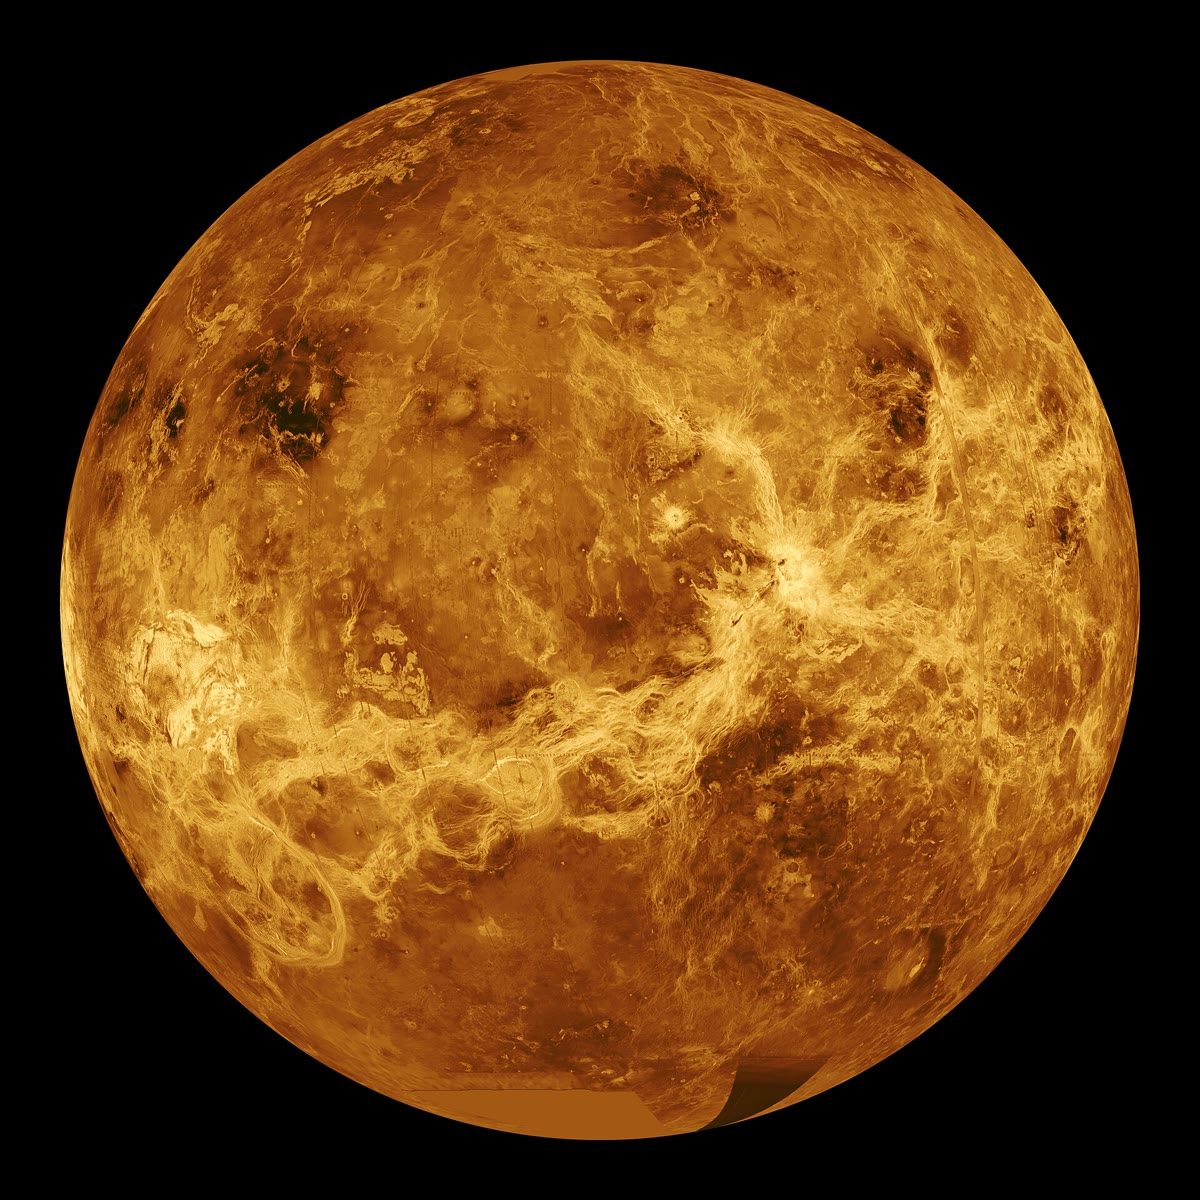
\includegraphics[width=\linewidth]{images/book3/b1-venus-radar-globe.jpg}
\end{minipage}\hspace{0.06\linewidth}
\begin{minipage}{0.4\linewidth}
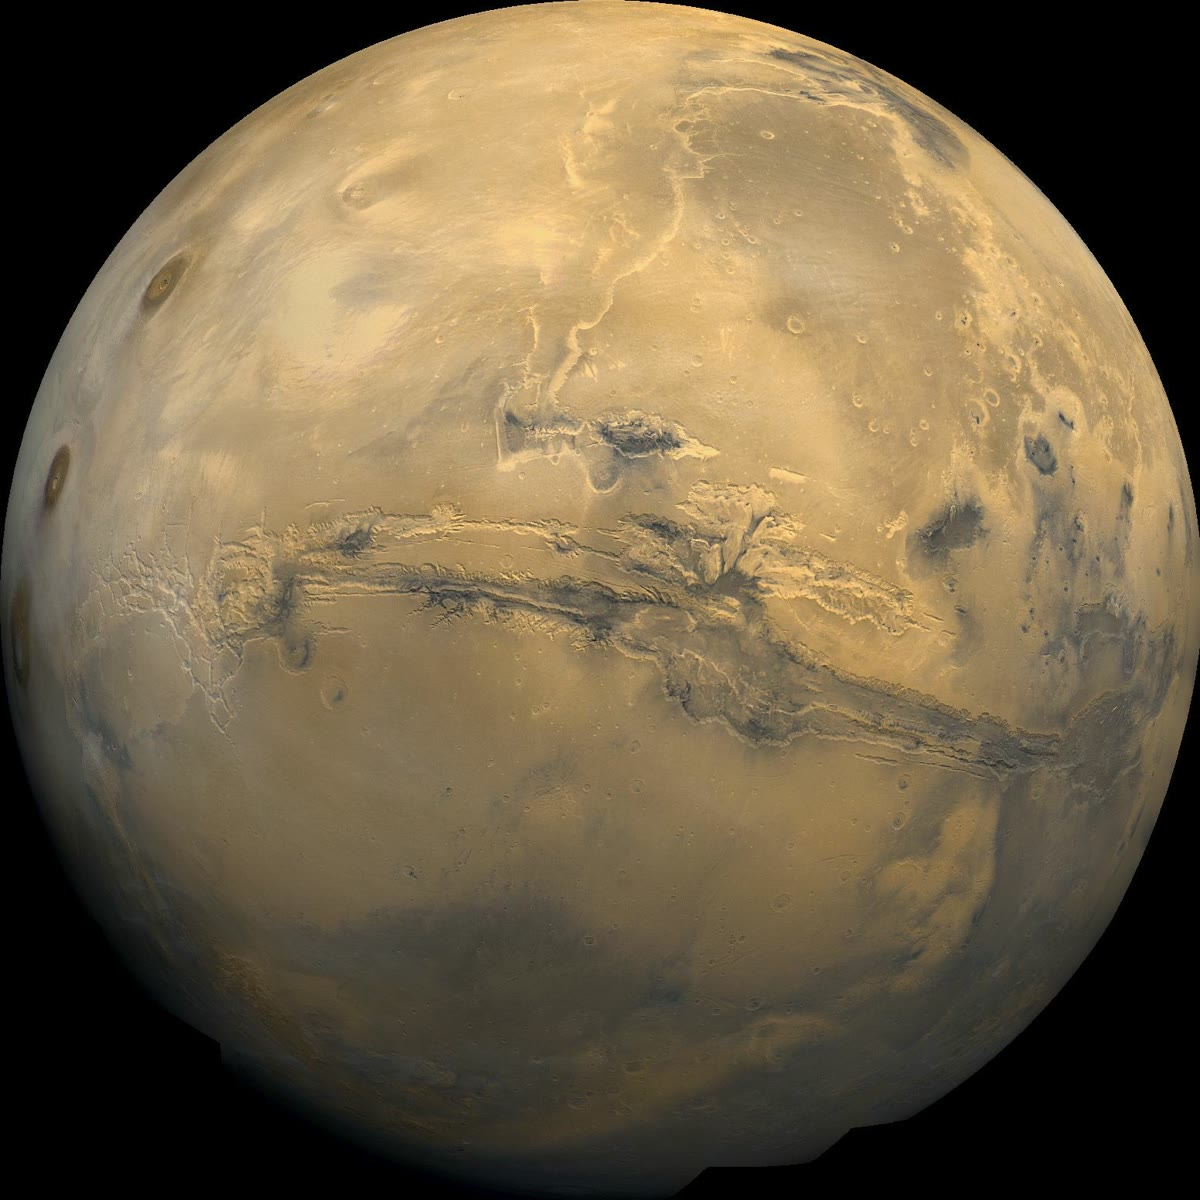
\includegraphics[width=\linewidth]{images/book3/b1-mars-valles-marineris.jpg}
\end{minipage}

{\small Left: the surface of Venus seen through its clouds by the radar of
the Magellan spacecraft, mapped onto a computer-simulated globe (the colours
are simulated). Right: Mars from the Viking 1 orbiter, a mosaic centred on
the canyon system of Valles Marineris. NASA/JPL and NASA/USGS, public
domain.}
% ledger: commons:venus-globe, commons:mars-valles
\end{omfigure}

The surfaces carry the record of what shaped them. Impact craters
accumulate on any surface exposed to space, so a heavily cratered surface,
like most of the Moon's or Mercury's, is old, and a surface with few
craters has been renewed: by lava flows, by erosion, or by the plates that
carry the Earth's ocean floor back into the mantle. Volcanic plains and
volcanoes are found on all the \omterm{def:b1:comparative-planetology:planet-types}{terrestrial planets}. Faults, rifts
and folded belts show that the lithospheres of Venus and Mars have been
deformed; but of all the planets, only the Earth shows today a lithosphere
broken into plates that move as rigid blocks, with ridges where they are
made and trenches where they sink. Why the Earth alone has plate tectonics
is still discussed; the presence of water, which weakens rocks, is one of
the reasons put forward.

\section{Moons and small bodies}

The Moon, a quarter of the Earth's diameter, is large for a satellite. Its
density, \qty{3340}{kg.m^{-3}}, close to that of the Earth's mantle rocks,
and its \omterm{def:b1:comparative-planetology:moi}{moment-of-inertia factor}, close to $0.4$, show that it has at most a
small iron core. The \omterm{def:b1:comparative-planetology:planet-types}{giant planets} have systems of moons that are worlds in
themselves (see the photographs below). Io, the innermost of Jupiter's four
large moons, is the most volcanically active world in the Solar System,
with hundreds of volcanoes, heated by the tides Jupiter raises in it;
volcanism resurfaces it faster than impacts can mark it with large craters.
Europa, of density \qty{3010}{kg.m^{-3}}, is rock under a crust of ice, and
there is strong evidence for a salty ocean beneath that crust. Ganymede and
Callisto, of densities \num{1940} and \qty{1830}{kg.m^{-3}}, are made of
rock and ice in comparable amounts.
Titan, Saturn's largest moon, is the only moon with a dense atmosphere,
mostly nitrogen with a little methane, and the only world besides the
Earth with rivers, lakes and seas on its surface --- of liquid methane and
ethane; it too probably hides an ocean of water.
% ledger: planet:Moon.diameter, planet:Earth.diameter, planet:Moon.density, nasa:moon, nasa:io-facts, nasa:europa, nasa:europa-facts, nasa:ganymede, nasa:titan-facts

\begin{omfigure}
\begin{minipage}{0.4\linewidth}
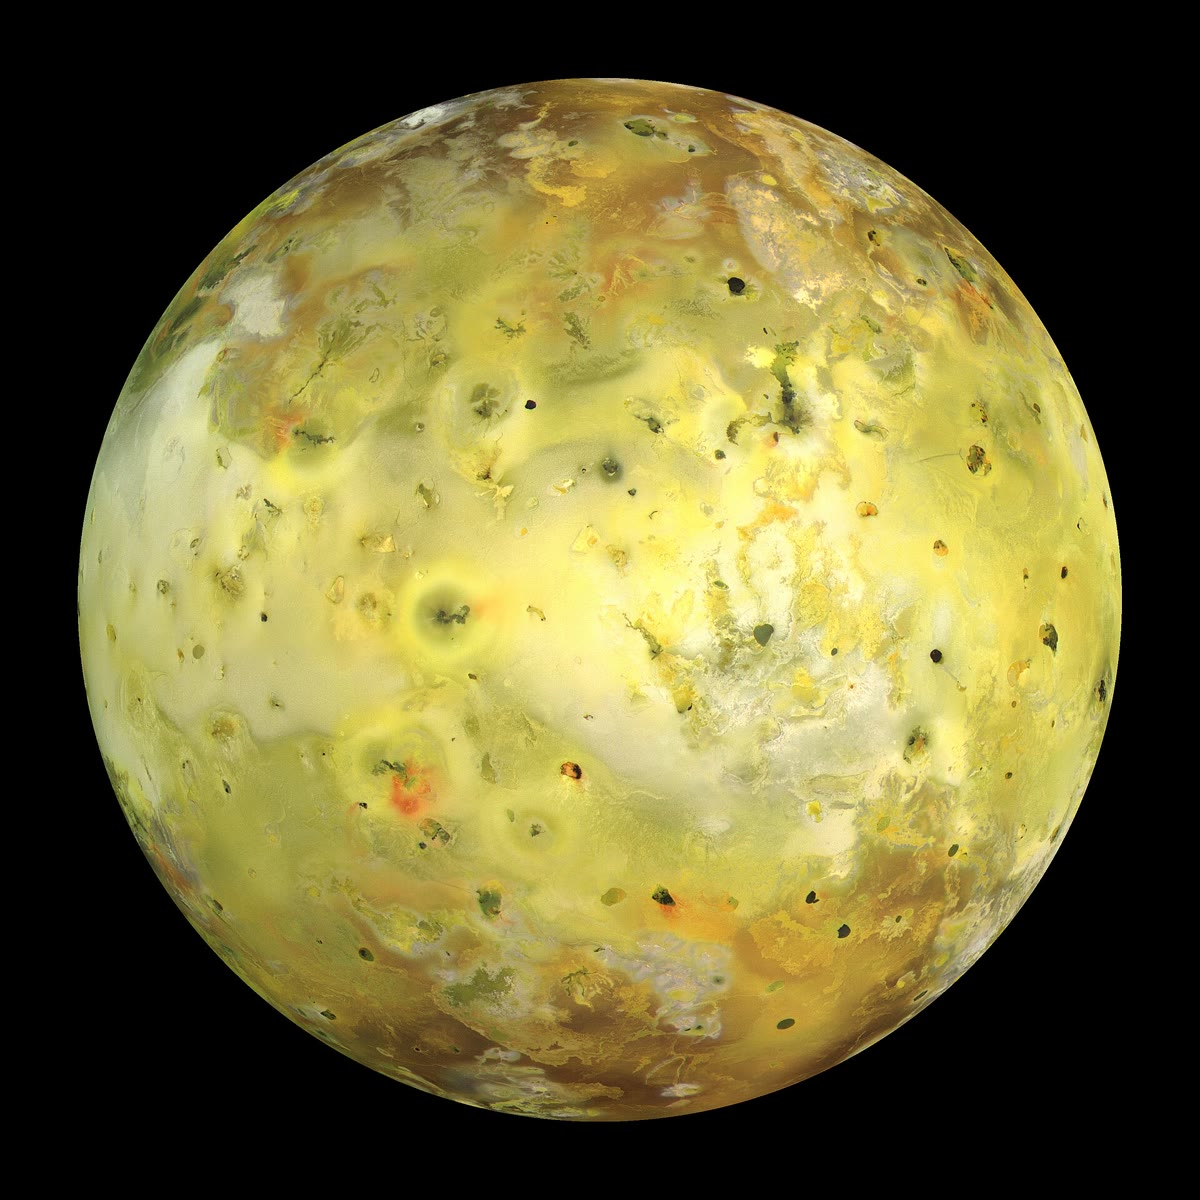
\includegraphics[width=\linewidth]{images/book3/b1-io.jpg}
\end{minipage}\hspace{0.06\linewidth}
\begin{minipage}{0.4\linewidth}
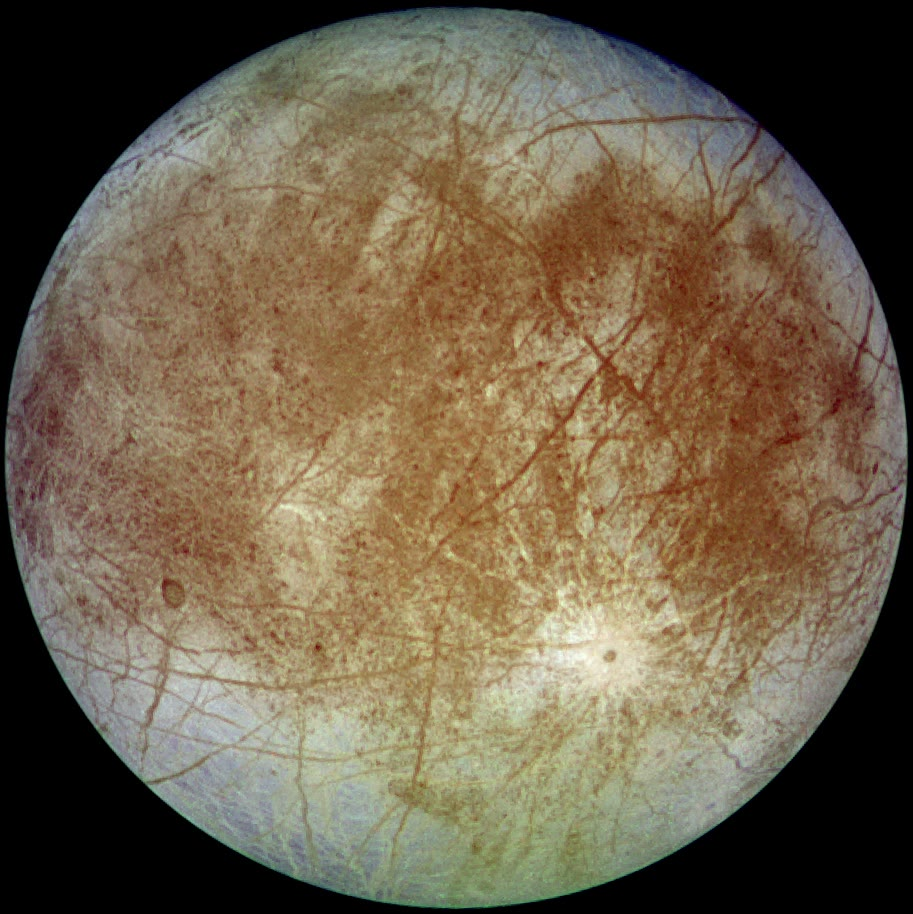
\includegraphics[width=\linewidth]{images/book3/b1-europa.jpg}
\end{minipage}

{\small Two of Jupiter's large moons seen by the Galileo spacecraft. Left:
Io, its surface dotted with volcanic centres and coloured by sulfur
compounds and lavas. Right: Europa in approximate natural colour; the long
dark lines are fractures in its icy crust. NASA/JPL/University of Arizona
and NASA/JPL/DLR, public domain.}
% ledger: commons:io, commons:europa, nasa:io-facts, nasa:europa
\end{omfigure}

\begin{definition}[Asteroid, comet, trans-Neptunian object]\label{def:b1:comparative-planetology:small-bodies}
An \emph{asteroid}\index{asteroid} is a small rocky or metallic body that
orbits the Sun, too small to be a planet and without the gas and dust
envelope of a comet; most orbit between Mars and Jupiter. A
\emph{comet}\index{comet} is a small body of ice and dust that, when its
orbit brings it near the Sun, releases gas and dust that form a glowing
envelope round it and tails pointing away from the Sun. A
\emph{trans-Neptunian object}\index{trans-Neptunian object} is a body of
the Solar System whose orbit lies, on average, beyond that of Neptune.
\end{definition}

The \omterm{def:b1:comparative-planetology:small-bodies}{trans-Neptunian objects} of the Kuiper Belt, a disc-shaped zone beyond
Neptune, are icy and rocky bodies left from the formation of the planets;
Pluto, classed as a dwarf planet since 2006, is one of them. The \omterm{def:b1:comparative-planetology:small-bodies}{asteroids} are
the debris of a region where no planet formed. Pieces of \omterm{def:b1:comparative-planetology:small-bodies}{asteroids}, and a
few of the Moon and Mars, fall on the Earth as meteorites. They are the
only samples of other worlds in our hands besides those brought back by
spacecraft, and some of them have changed little since the Solar System
formed; their classes, and what they say about the composition of the Earth
and the age of the Solar System, are the subject of the Year~2 volume.
% ledger: nasa:pluto-facts

\section{Exercises}

\begin{exercise}[$\star$]\label{exo:b1:comparative-planetology:1}
Jupiter has a mass of \qty{1898.13e24}{kg} and a mean radius of
\qty{69911}{km}. Compute its mean density and compare it with that of water,
\qty{1000}{kg.m^{-3}}.
\end{exercise}

\begin{exercise}[$\star$]\label{exo:b1:comparative-planetology:2}
Using the figure of densities and radii, classify Mercury, Saturn, Uranus and
Venus as \omterm{def:b1:comparative-planetology:planet-types}{terrestrial planets}, \omterm{def:b1:comparative-planetology:planet-types}{gas giants} or \omterm{def:b1:comparative-planetology:planet-types}{ice giants}, and justify each
choice by its radius and density.
\end{exercise}

\begin{exercise}[$\star$]\label{exo:b1:comparative-planetology:3}
Venus receives \qty{2601.3}{W.m^{-2}} and has a \omterm{def:b1:comparative-planetology:albedo}{Bond albedo} of 0.77.
Compute its \omterm{def:b1:comparative-planetology:equilibrium-temperature}{equilibrium temperature}. Why is it lower than the Earth's,
although Venus is nearer the Sun?
\end{exercise}

\begin{exercise}[$\star$]\label{exo:b1:comparative-planetology:4}
Rank the Moon ($C = 0.394$), Mars (0.366), the Earth (0.3308), Jupiter
(0.254) and Saturn (0.210) from the most uniform to the most centrally
concentrated. What would $C$ be for a planet whose whole mass sat in a point
at its centre?
\end{exercise}

\begin{exercise}[$\star\star$]\label{exo:b1:comparative-planetology:5}
Titan orbits Saturn at $a = \qty{1221.87e3}{km}$ in \num{15.945421} days.
Compute the mass of Saturn and compare it with the tabulated
\qty{568.32e24}{kg}.
\end{exercise}

\begin{exercise}[$\star\star$]\label{exo:b1:comparative-planetology:6}
The Earth receives \qty{1361}{W.m^{-2}} at \qty{149.6e6}{km} from the Sun.
Compute the irradiance at Mars (\qty{228.0e6}{km}) and at Jupiter
(\qty{778.5e6}{km}), and compare with the tabulated \qty{586.2}{W.m^{-2}}
and \qty{50.26}{W.m^{-2}}.
\end{exercise}

\begin{exercise}[$\star\star$]\label{exo:b1:comparative-planetology:7}
Show that, for a given albedo, $T_\mathrm{eq}$ varies as $d^{-1/2}$. Compute
$T_\mathrm{eq}$ for Jupiter ($S = \qty{50.26}{W.m^{-2}}$, $A = 0.343$).
If Jupiter were found to radiate more power than it absorbs from the Sun,
what would that imply about its interior?
\end{exercise}

\begin{exercise}[$\star\star$]\label{exo:b1:comparative-planetology:8}
Compute the greenhouse warming $T_\mathrm{surf} - T_\mathrm{eq}$ of Venus
(\qty{737}{K}), the Earth (\qty{288}{K}, $A = 0.294$) and Mars
(\qty{214}{K}). Express each as a fraction of $T_\mathrm{eq}$.
\end{exercise}

\begin{exercise}[$\star\star$]\label{exo:b1:comparative-planetology:9}
For a uniform sphere, show that $C = 0.4$ by integrating the moments of
inertia of thin spherical shells (a shell of radius $r$ and mass
$\mathrm dm$ has $\mathrm dI = \tfrac23 r^2\,\mathrm dm$). What value does a
hollow shell of radius $R$ have?
\end{exercise}

\begin{exercise}[$\star\star\star$]\label{exo:b1:comparative-planetology:10}
Mercury has $\bar\rho = \qty{5429}{kg.m^{-3}}$, $C = 0.35$ and a radius of
\qty{2439.7}{km}. With a mantle density of \qty{3300}{kg.m^{-3}}, use the
two-layer model to find its core radius, its core density and the fraction
of its mass in the core. What is remarkable about Mercury?
\end{exercise}

\begin{exercise}[$\star\star\star$]\label{exo:b1:comparative-planetology:11}
Model an airless body whose day hemisphere is at the uniform temperature
$T_1$ and night hemisphere at $T_2$, radiating together the absorbed power.
(a) Show that if $T_1^4 + T_2^4 = 2T_\mathrm{eq}^4$, the mean temperature
$(T_1 + T_2)/2$ is at most $T_\mathrm{eq}$, with equality only when
$T_1 = T_2$. (b) For the Moon, $T_\mathrm{eq} = \qty{270}{K}$; take
$T_2 = \qty{100}{K}$. Compute $T_1$ and the mean temperature.
\end{exercise}

\begin{exercise}[$\star\star\star$]\label{exo:b1:comparative-planetology:12}
Venus has a radius of \qty{6051.8}{km}, a surface gravity of
\qty{8.9}{m.s^{-2}} and a surface pressure of \qty{92}{bar}. Compute the
mass of its atmosphere, compare it with the Earth's, \qty{5.1e18}{kg}, and
with the mass of Venus, \qty{4.8673e24}{kg}. What does the comparison
suggest about where the Earth's carbon dioxide is kept?
% ledger: earth:Matm, planet:Venus.gravity, nasa:venus
\end{exercise}

\section{Problem: Weighing and sounding Mars}

\begin{problem}[{Weekend problem --- the mass of Mars from its moon, its
density and temperature, and the size of its core}]
\label{pb:b1:comparative-planetology:1}
% ledger: nasa:phobos, nasa:mars, nasa:mars-core, const:G, const:sigma, earth:psurf, earth:gmean, planet:Mars.Prot, planet:Earth.density
% numbers computed in the scratch calculator calc/ch03.py from the rounded data
Phobos, the larger moon of Mars, orbits at a mean distance of
\qty{9378}{km} from the centre of Mars in \num{0.31891} days. Mars has a mean
radius of \qty{3389.5}{km}, a rotation period of \qty{24.6}{h}, a
\omterm{def:b1:comparative-planetology:moi}{moment-of-inertia factor} $C = 0.366$, a \omterm{def:b1:comparative-planetology:albedo}{Bond albedo} of 0.250 and a mean
surface pressure of \qty{6.36}{mbar}; it receives \qty{586.2}{W.m^{-2}} from
the Sun, and its mean surface temperature is about \qty{214}{K}. Phobos has
a mass of \qty{1.06e16}{kg}. Take $G = \qty{6.6743e-11}{m^3.kg^{-1}.s^{-2}}$
and $\sigma = \qty{5.6704e-8}{W.m^{-2}.K^{-4}}$.

\medskip
\noindent\textbf{Part I --- Weighing Mars.}
\begin{enumerate}
  \item Convert the period of Phobos to seconds.
  \item Compute $GM$ for Mars.
  \item Deduce the mass of Mars.
  \item Is it right to neglect the mass of Phobos?
  \item Compute the orbital speed of Phobos.
  \item Compare the period of Phobos with the rotation of Mars. In which
        direction does Phobos cross the sky of Mars?
\end{enumerate}

\medskip
\noindent\textbf{Part II --- Density and gravity.}
\begin{enumerate}[resume]
  \item Compute the volume of Mars.
  \item Compute its mean density, rounded to \qty{10}{kg.m^{-3}}.
  \item Compare it with the Earth's, \qty{5514}{kg.m^{-3}}. Give two
        reasons why the Earth is denser.
  \item Compute the gravity at the surface of Mars.
  \item Compute the escape velocity from the surface of Mars.
\end{enumerate}

\medskip
\noindent\textbf{Part III --- Temperature and atmosphere.}
\begin{enumerate}[resume]
  \item Compute the \omterm{def:b1:comparative-planetology:equilibrium-temperature}{equilibrium temperature} of Mars.
  \item Compare it with the mean surface temperature. How large is the
        greenhouse warming?
  \item Compute the mass of the atmosphere above each square metre of Mars,
        and compare it with the Earth's ($p = \qty{1014}{hPa}$,
        $g = \qty{9.82}{m.s^{-2}}$).
  \item Compute the total mass of the atmosphere of Mars.
  \item Mars's atmosphere is \qty{95}{\percent} carbon dioxide, yet its
        greenhouse warming is small. Suggest why.
\end{enumerate}

\medskip
\noindent\textbf{Part IV --- The core of Mars.}
\begin{enumerate}[resume]
  \item What would $C$ be if Mars were uniform? What does the measured
        value tell?
  \item Write the mean density of a two-layer Mars in terms of the relative
        core radius $x$, the mantle density $\rho_m$ and the core density
        $\rho_c$.
  \item Write its \omterm{def:b1:comparative-planetology:moi}{moment-of-inertia factor} in the same terms.
  \item Show that $x^2 = (\tfrac52C\bar\rho - \rho_m)/(\bar\rho - \rho_m)$.
  \item With the mean density of question 8 and $\rho_m =
        \qty{3500}{kg.m^{-3}}$, compute $x$ and the core density.
  \item What fraction of the mass of Mars is in its core?
  \item Repeat question 21 with $\rho_m = 3450$ and
        \qty{3550}{kg.m^{-3}}. What do you conclude about the precision of
        the model?
  \item Give the radius of the core of Mars from the model with
        $\rho_m = \qty{3500}{kg.m^{-3}}$, and compare it with the value of
        the planetary table, \qty{1830}{km}, and with the recent seismic
        result, \qty{1650}{km} to \qty{1675}{km}.
\end{enumerate}
\end{problem}
